\section{Results}\label{sec:results}

Figure~\ref{fig:forest} summarizes the HOTA difference between each host with
\scl{} and the host alone for every evaluated cell. The following
subsections give the baseline comparison for each part of the evaluation.

\begin{figure}[t]
\centering
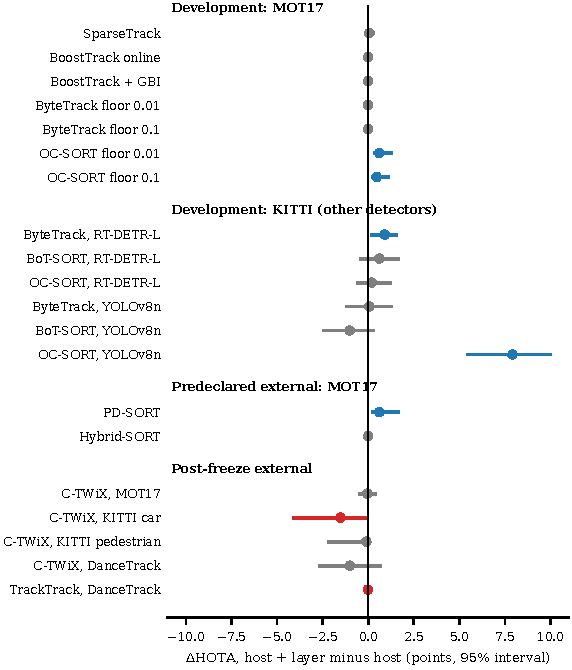
\includegraphics[width=\columnwidth]{figures/fig3_forest_col.pdf}
\caption{Difference in HOTA (host with \scl{} minus host alone) with
95\% paired-bootstrap interval for every evaluated cell. Blue: above zero;
red: below zero; gray: includes zero or identical output.}
\label{fig:forest}
\end{figure}

\subsection{Tracker transfer}\label{sec:tracker}
Table~\ref{tab:mot17} compares the development trackers with their hosts on
MOT17. The two-stage trackers with well-matched detections stayed at the
accuracy of their hosts. BoostTrack, online and with interpolation, and
ByteTrack at floor 0.1 produced identical output. ByteTrack at floor 0.01
changed by $-0.014$ HOTA and SparseTrack by $+0.055$. This is the
self-limiting behavior of the clean regime (Sect.~\ref{sec:regimes}), which
the prior design did not have (Table~\ref{tab:prior}).

The single-stage OC-SORT improved at both emission floors. Its HOTA rose by
0.61 points ($[+0.36,+1.24]$) at floor 0.01 and by 0.46 points
($[+0.27,+1.09]$) at floor 0.1, and its MOTA by 1.27 and 1.26 points. HOTA
was higher on 7 of 7 sequences in both settings (Fig.~\ref{fig:perseq}). The
gain comes from the continuation rescue. OC-SORT discards every detection
below its single threshold, and the layer passes it the foreground candidates
that continue a track that would otherwise stay unmatched.

\begin{table}[t]
\caption{Baseline comparison of the development trackers on MOT17 val-half
(published YOLOX-X detections). Paper: number reported by the tracker's
authors. Host: published tracker alone (our reproduction). $\Delta$: host with
\scl{} minus host, with 95\% paired-bootstrap interval (10,000
resamples, seed 42); bold intervals exclude zero. The floor is the lowest
detector score emitted.}
\label{tab:mot17}
\centering\footnotesize
\setlength{\tabcolsep}{4pt}
\begin{tabular}{@{}lrrl@{}}
\toprule
Metric & Paper & Host & $\Delta$ [95\% CI]\\
\midrule
\multicolumn{4}{@{}l}{\textit{SparseTrack} \cite{liu2025sparsetrack}}\\
\quad HOTA & 69.2 & 68.88 & $+0.06$ [$-0.01$, $+0.25$]\\
\quad MOTA & 76.8 & 77.85 & $+0.08$ [$-0.03$, $+0.30$]\\
\quad IDF1 & 81.4 & 81.97 & $+0.16$ [$-0.02$, $+0.70$]\\
\multicolumn{4}{@{}l}{\textit{BoostTrack, online} \cite{stanojevic2024boosttrack}}\\
\quad HOTA & 68.37 & 68.49 & 0 (identical)\\
\quad MOTA & 75.56 & 75.50 & 0 (identical)\\
\quad IDF1 & 81.35 & 81.41 & 0 (identical)\\
\multicolumn{4}{@{}l}{\textit{BoostTrack, + GBI} \cite{stanojevic2024boosttrack}}\\
\quad HOTA & 71.33 & 71.72 & 0 (identical)\\
\quad MOTA & 80.55 & 81.03 & 0 (identical)\\
\quad IDF1 & 83.84 & 84.16 & 0 (identical)\\
\multicolumn{4}{@{}l}{\textit{ByteTrack, floor 0.01} \cite{zhang2022bytetrack}}\\
\quad HOTA & -- & 67.70 & $-0.014$ [$-0.058$, $+0.009$]\\
\quad MOTA & 76.6 & 77.60 & $+0.06$ [$-0.15$, $+0.34$]\\
\quad IDF1 & 79.3 & 79.47 & $-0.031$ [$-0.135$, $+0.035$]\\
\multicolumn{4}{@{}l}{\textit{ByteTrack, floor 0.1} \cite{zhang2022bytetrack}}\\
\quad HOTA & -- & 67.70 & 0 (identical)\\
\quad MOTA & 76.6 & 77.60 & 0 (identical)\\
\quad IDF1 & 79.3 & 79.47 & 0 (identical)\\
\multicolumn{4}{@{}l}{\textit{OC-SORT, floor 0.01} \cite{cao2023ocsort}}\\
\quad HOTA & 66.5 & 66.43 & {\boldmath $+0.61$ [$+0.36$, $+1.24$]}\\
\quad MOTA & 74.9 & 74.67 & {\boldmath $+1.27$ [$+0.17$, $+3.01$]}\\
\quad IDF1 & 77.7 & 78.05 & $+0.66$ [$-0.25$, $+1.60$]\\
\multicolumn{4}{@{}l}{\textit{OC-SORT, floor 0.1} \cite{cao2023ocsort}}\\
\quad HOTA & 66.5 & 66.44 & {\boldmath $+0.46$ [$+0.27$, $+1.09$]}\\
\quad MOTA & 74.9 & 74.67 & {\boldmath $+1.26$ [$+0.37$, $+3.34$]}\\
\quad IDF1 & 77.7 & 78.05 & {\boldmath $+0.287$ [$+0.003$, $+0.838$]}\\
\bottomrule
\end{tabular}
\end{table}


\begin{figure}[t]
\centering
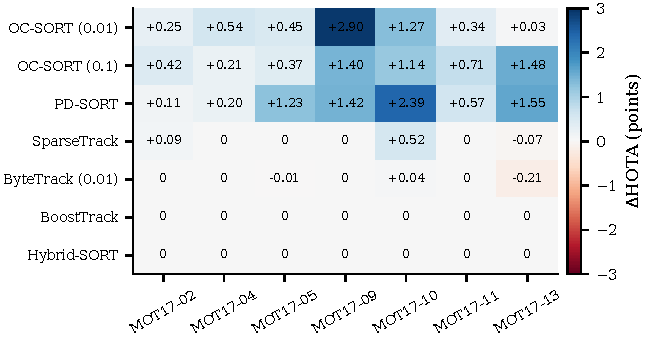
\includegraphics[width=\columnwidth]{figures/fig4_per_sequence.pdf}
\caption{Per-sequence HOTA differences (host with \scl{} minus host
alone) on MOT17 val-half for the development and predeclared trackers.}
\label{fig:perseq}
\end{figure}

\subsection{Detector change}\label{sec:detector}
Table~\ref{tab:kitti} reports three trackers with two detectors on KITTI. With
the noisy RT-DETR-L stream, the two-stage trackers gained in MOTA and IDF1.
ByteTrack gained 5.98 MOTA points ($[+1.16,+9.94]$), 3.87 IDF1 points, and
0.91 HOTA points ($[+0.22,+1.55]$). BoT-SORT gained 7.86 MOTA points
($[+2.21,+13.44]$) and 3.10 IDF1 points. With YOLOv8n, the single-stage
OC-SORT gained 7.91 HOTA points ($[+5.47,+9.98]$), 9.40 MOTA points, and 9.60
IDF1 points.

\begin{table}[t]
\caption{Baseline comparison under a detector change on KITTI tracking
training (official HOTA, car and pedestrian averaged). Host: published
tracker alone with the same detections. $\Delta$: host with \scl{}
minus host, with 95\% paired-bootstrap interval; bold intervals exclude zero.
BoT-SORT excludes one sequence on which the unmodified tracker fails
numerically.}
\label{tab:kitti}
\centering\footnotesize
\setlength{\tabcolsep}{4pt}
\begin{tabular}{@{}lrl@{}}
\toprule
Metric & Host & $\Delta$ [95\% CI]\\
\midrule
\multicolumn{3}{@{}l}{\textit{ByteTrack} \cite{zhang2022bytetrack}\textit{, RT-DETR-L}}\\
\quad HOTA & 50.73 & {\boldmath $+0.91$ [$+0.22$, $+1.55$]}\\
\quad MOTA & 47.27 & {\boldmath $+5.98$ [$+1.16$, $+9.94$]}\\
\quad IDF1 & 64.98 & {\boldmath $+3.87$ [$+1.67$, $+5.06$]}\\
\multicolumn{3}{@{}l}{\textit{BoT-SORT} \cite{aharon2022botsort}\textit{, RT-DETR-L}}\\
\quad HOTA & 53.91 & $+0.61$ [$-0.39$, $+1.61$]\\
\quad MOTA & 48.25 & {\boldmath $+7.86$ [$+2.21$, $+13.44$]}\\
\quad IDF1 & 67.74 & {\boldmath $+3.10$ [$+1.00$, $+4.57$]}\\
\multicolumn{3}{@{}l}{\textit{OC-SORT} \cite{cao2023ocsort}\textit{, RT-DETR-L}}\\
\quad HOTA & 52.64 & $+0.19$ [$-0.57$, $+1.19$]\\
\quad MOTA & 57.59 & $-0.57$ [$-4.36$, $+1.40$]\\
\quad IDF1 & 69.87 & $+0.04$ [$-1.31$, $+1.78$]\\
\multicolumn{3}{@{}l}{\textit{ByteTrack} \cite{zhang2022bytetrack}\textit{, YOLOv8n}}\\
\quad HOTA & 45.31 & $+0.06$ [$-1.19$, $+1.24$]\\
\quad MOTA & 46.54 & $-1.87$ [$-6.25$, $+0.03$]\\
\quad IDF1 & 60.92 & $+1.49$ [$-0.36$, $+3.27$]\\
\multicolumn{3}{@{}l}{\textit{BoT-SORT} \cite{aharon2022botsort}\textit{, YOLOv8n}}\\
\quad HOTA & 49.21 & $-1.02$ [$-2.43$, $+0.25$]\\
\quad MOTA & 49.89 & {\boldmath $-2.43$ [$-7.43$, $-0.14$]}\\
\quad IDF1 & 64.41 & $+0.35$ [$-2.10$, $+2.27$]\\
\multicolumn{3}{@{}l}{\textit{OC-SORT} \cite{cao2023ocsort}\textit{, YOLOv8n}}\\
\quad HOTA & 36.27 & {\boldmath $+7.91$ [$+5.47$, $+9.98$]}\\
\quad MOTA & 33.99 & {\boldmath $+9.40$ [$+1.10$, $+12.30$]}\\
\quad IDF1 & 50.46 & {\boldmath $+9.60$ [$+5.61$, $+12.16$]}\\
\bottomrule
\end{tabular}
\end{table}


\subsection{Detector confidence shift}\label{sec:shift}
Table~\ref{tab:shift} and Fig.~\ref{fig:shift} give the trackers under the
four score transforms. Halving the scores drove ByteTrack (official setting)
and OC-SORT to 0 HOTA, because no detection reached their thresholds. With the
layer they reached 66.17 and 66.72. Cubing reduced them to 60.92 and 58.34,
and the layer restored them to 65.81 and 66.60. BoostTrack rose from 61.33 to
64.84 under cubing. With temperature $T=2$, the layer raised ByteTrack and
OC-SORT by 1.11 and 1.24 points. The library setting of ByteTrack, whose low
thresholds already admit the shifted scores, stayed within 0.14 points in all
four transforms. Over the 14 conditions, the layer raised HOTA significantly
in 7 and lowered it significantly in none.

\begin{table}[t]
\caption{Baseline comparison under detector confidence shift on MOT17 val-half
(HOTA). The detector scores are transformed before the tracker, whose
published thresholds stay fixed; $T$ is a logit temperature, $\sigma(z/T)$.
Host: published tracker alone. $\Delta$: with \scl{} minus host,
with 95\% paired-bootstrap interval (10,000 resamples, seed 42). Bold
intervals exclude zero. Emission floor 0.01 (BoostTrack 0.1).}
\label{tab:shift}
\centering\footnotesize
\setlength{\tabcolsep}{4pt}
\begin{tabular}{@{}lrrl@{}}
\toprule
Transform & Host & + \scl{} & $\Delta$HOTA\\
\midrule
\multicolumn{4}{@{}l}{\textit{ByteTrack, official setting} \cite{zhang2022bytetrack}}\\
\quad $s^3$ & 60.92 & 65.81 & {\boldmath $+4.89$ [$+2.60$, $+13.69$]}\\
\quad $0.5\,s$ & 0.00 & 66.17 & {\boldmath $+66.17$ [$+49.32$, $+75.40$]}\\
\quad $T=2$ & 65.84 & 66.95 & {\boldmath $+1.11$ [$+0.35$, $+3.87$]}\\
\quad $T=0.5$ & 67.30 & 67.29 & $-0.009$ [$-0.051$, $+0.005$]\\
\multicolumn{4}{@{}l}{\textit{ByteTrack, library setting} \cite{zhang2022bytetrack}}\\
\quad $s^3$ & 66.31 & 66.31 & $-0.006$ [$-0.384$, $+0.383$]\\
\quad $0.5\,s$ & 66.61 & 66.48 & $-0.14$ [$-0.66$, $+0.14$]\\
\quad $T=2$ & 63.97 & 63.97 & 0 (identical)\\
\quad $T=0.5$ & 66.53 & 66.52 & $-0.006$ [$-0.029$, $+0.001$]\\
\multicolumn{4}{@{}l}{\textit{OC-SORT} \cite{cao2023ocsort}}\\
\quad $s^3$ & 58.34 & 66.60 & {\boldmath $+8.26$ [$+5.86$, $+16.81$]}\\
\quad $0.5\,s$ & 0.00 & 66.72 & {\boldmath $+66.72$ [$+50.32$, $+75.56$]}\\
\quad $T=2$ & 65.99 & 67.22 & {\boldmath $+1.24$ [$+0.52$, $+3.42$]}\\
\quad $T=0.5$ & 66.61 & 67.06 & $+0.45$ [$-0.01$, $+0.97$]\\
\multicolumn{4}{@{}l}{\textit{BoostTrack, online} \cite{stanojevic2024boosttrack}}\\
\quad $s^3$ & 61.33 & 64.84 & {\boldmath $+3.51$ [$+0.85$, $+13.28$]}\\
\quad $T=2$ & 67.59 & 67.59 & 0 (identical)\\
\bottomrule
\end{tabular}
\end{table}


\begin{figure*}[t]
\centering
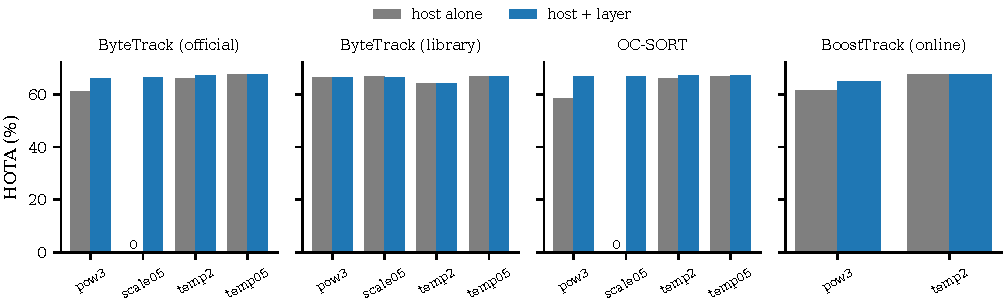
\includegraphics[width=0.9\textwidth]{figures/fig5_calibration_shift.pdf}
\caption{Detector confidence shift on MOT17 val-half: HOTA of each published
tracker with its published thresholds, alone and with \scl{}, after
four monotone transforms of the detector scores (pow3: $s^3$; scale05:
$0.5\,s$; temp2 and temp05: $T=2$ and $T=0.5$).}
\label{fig:shift}
\end{figure*}

\subsection{External systems}\label{sec:external}
Table~\ref{tab:external} gives every external system. PD-SORT
\cite{wang2025pdsort} was reproduced identically to the authors' released
output. With \scl{}, its HOTA rose by 0.61 points ($[+0.27,+1.65]$), its
MOTA by 1.13 points ($[+0.27,+3.03]$), and its IDF1 by 0.82 points
($[+0.43,+1.94]$), with higher HOTA on 7 of 7 sequences
(Fig.~\ref{fig:perseq}). False negatives fell by 1,291, and false positives
rose by 681. PD-SORT is a single-stage tracker, and its gain follows the same
mechanism as for OC-SORT; unlike OC-SORT, it was not seen during design.
Hybrid-SORT \cite{yang2024hybridsort}, a two-stage tracker, produced identical
output, as predicted before the run.

After the freeze, C-TWiX \cite{miah2025twix} was reproduced on three datasets
and TrackTrack \cite{shim2025tracktrack} on DanceTrack, all within the
reproduction criterion. Their results are listed in Table~\ref{tab:external}. On
DanceTrack, the output of TrackTrack with \scl{} was tied with the host on
21 of 25 sequences.

\begin{table*}[t]
\caption{Baseline comparison on the external systems, each evaluated once with
the frozen \scl{}. Reference / reproduced: the authors' HOTA and the HOTA of
the host alone in our runs. Reproduction class against the authors' number
(EXACT: $|\Delta\mathrm{HOTA}|\le0.2$; CLOSE: $\le1.0$ with a documented,
untuned cause). $\Delta$: host with \scl{} minus host, with 95\%
paired-bootstrap interval; bold intervals exclude zero. TOPICTrack failed
reproduction and is excluded from the analysis.}
\label{tab:external}
\centering\footnotesize
\setlength{\tabcolsep}{4pt}
\begin{tabular}{@{}lccccc@{}}
\toprule
System & Reference / & Class & $\Delta$HOTA & $\Delta$MOTA & $\Delta$IDF1\\
(data) & reproduced & & & & \\
\midrule
\multicolumn{6}{@{}l}{\textit{Predeclared before the runs}}\\
\twol{PD-SORT \cite{wang2025pdsort}}{MOT17 val-half} & 68.01 / 68.01 & \twol{EXACT}{(released output)} & \cib{+0.61}{+0.27}{+1.65} & \cib{+1.13}{+0.27}{+3.03} & \cib{+0.82}{+0.43}{+1.94}\\[6pt]
\twol{Hybrid-SORT \cite{yang2024hybridsort}}{MOT17 val-half} & 67.1 / 66.70 & CLOSE & 0 (identical) & 0 (identical) & 0 (identical)\\[2pt]
\multicolumn{6}{@{}l}{\textit{Post-freeze, protocol registered before the runs}}\\
\twol{C-TWiX \cite{miah2025twix}}{MOT17 val-half} & 77.8 / 77.55 & CLOSE & \ci{-0.05}{-0.46}{+0.40} & \ci{+0.24}{-0.58}{+1.12} & \ci{+0.18}{-0.47}{+1.14}\\[6pt]
\twol{C-TWiX (car)}{KITTI MOTS val} & 89.3 / 89.27 & EXACT & \cib{-1.52}{-4.05}{-0.13} & \cib{-2.11}{-5.89}{-0.17} & \cib{-1.21}{-3.32}{-0.10}\\[6pt]
\twol{C-TWiX (pedestrian)}{KITTI MOTS val} & 71.4 / 70.77 & CLOSE & \ci{-0.10}{-2.16}{+0.03} & \ci{-0.31}{-4.86}{+0.10} & \ci{-0.01}{-1.90}{+0.08}\\[6pt]
\twol{C-TWiX}{DanceTrack val} & 60.4 / 59.62 & CLOSE & \ci{-1.00}{-2.62}{+0.65} & \ci{+0.13}{-0.39}{+0.47} & \ci{-1.55}{-3.76}{+0.52}\\[6pt]
\twol{TOPICTrack \cite{cao2025topictrack}}{MOT17 val-half} & 69.6 / 67.54 & FAILED & \multicolumn{3}{c}{not analyzed}\\[2pt]
\twol{TrackTrack \cite{shim2025tracktrack}}{DanceTrack val} & 63.3 / 62.96 & CLOSE & \cib{-0.013}{-0.032}{-0.001} & \cib{-0.073}{-0.208}{-0.004} & \ci{+0.009}{-0.001}{+0.028}\\
\bottomrule
\end{tabular}
\end{table*}


\subsection{Latency}\label{sec:latency}
Table~\ref{tab:runtime} and Fig.~\ref{fig:runtime} compare the per-frame time
of the host pipeline with and without \scl{}. \scl{} took 2.95 ms per
frame on average and 4.39 ms at the 95th percentile, including the
phase-correlation motion cue. The end-to-end time rose from 57.85 to 60.44 ms
per frame, by 4.5\%. The tracker became faster, from 2.04 to 1.43 ms per
frame, because it received fewer candidates. The detector takes most of each
frame, about 42 ms, so the layer adds only a small part of the total latency.

\begin{table}[t]
\caption{Baseline comparison of the per-frame time on a 4-vCPU Intel Xeon
(2.10 GHz, no GPU) with a live YOLOv8n detector (736 pixels) and ByteTrack on
three KITTI sequences (2,279 timed frames per arm). Host alone: the same
pipeline without \scl{}. Mean / 95th percentile in milliseconds.}
\label{tab:runtime}
\centering\footnotesize
\setlength{\tabcolsep}{4pt}
\begin{tabular}{@{}lcc@{}}
\toprule
Stage & Host alone & Host + \scl{}\\
\midrule
Frame decode & 13.88 / 16.21 & 13.88 / 16.51\\
Detector (YOLOv8n, 736 px) & 41.91 / 58.41 & 42.17 / 59.43\\
\scl{} & -- & 2.95 / 4.39\\
Tracker (ByteTrack) & 2.04 / 3.57 & 1.43 / 2.64\\
End to end & 57.85 / 76.35 & 60.44 / 80.78\\
\bottomrule
\end{tabular}
\end{table}


\begin{figure}[t]
\centering
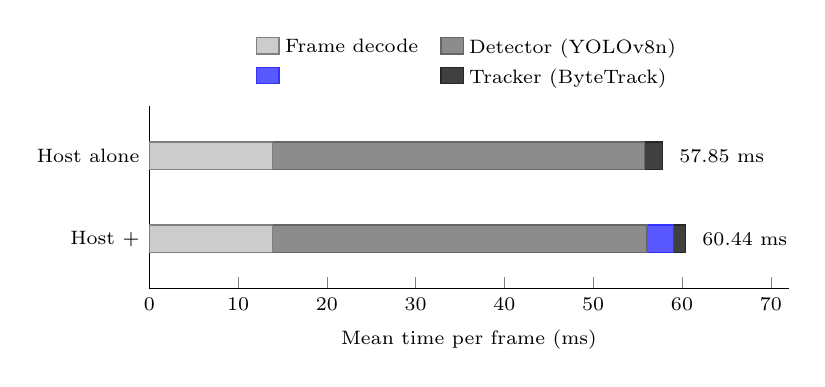
\begin{tikzpicture}
\begin{axis}[
  xbar stacked,
  /pgf/bar width=10pt,
  width=0.8\columnwidth,
  height=3.9cm,
  xmin=0, xmax=72,
  clip=false,
  ymin=-0.6, ymax=1.6,
  ytick={0,1},
  yticklabels={Host + \scl{}, Host alone},
  xlabel={Mean time per frame (ms)},
  axis x line*=bottom,
  axis y line*=left,
  tick label style={font=\scriptsize},
  label style={font=\scriptsize},
  legend style={at={(0.5,1.04)}, anchor=south, legend columns=2,
    font=\scriptsize, draw=none, /tikz/every even column/.append style={column sep=6pt}},
  legend cell align=left,
]
\addplot[fill=black!20, draw=black!50] coordinates {(13.88,1) (13.88,0)};
\addplot[fill=black!45, draw=black!60] coordinates {(41.91,1) (42.17,0)};
\addplot[fill=blue!65, draw=blue!80] coordinates {(0,1) (2.95,0)};
\addplot[fill=black!75, draw=black!85] coordinates {(2.04,1) (1.43,0)};
\legend{Frame decode, Detector (YOLOv8n), \scl{}, Tracker (ByteTrack)}
\node[anchor=west, font=\scriptsize] at (axis cs:58.6,1) {57.85 ms};
\node[anchor=west, font=\scriptsize] at (axis cs:61.2,0) {60.44 ms};
\end{axis}
\end{tikzpicture}

\caption{Mean per-frame time by stage for the host pipeline alone and with
\scl{} (4-vCPU Intel Xeon, no GPU). The labels give the measured
end-to-end time.}
\label{fig:runtime}
\end{figure}
